\documentclass{article}

% Packages
\usepackage[utf8]{inputenc} % For modern characters
\usepackage{microtype} % For sexy kerning
\usepackage{mathtools} % For math stuff
\usepackage{amssymb} % For math symbols
\usepackage{tabularx} % For making tables
\usepackage{listings} % For writing code
\usepackage{fancyhdr} % Use a header
\usepackage{pdfpages} % Include PDFs

% Set the margins
\usepackage[scale=0.8, top=1in, bottom=1in]{geometry}

% Other front matter
\lstset{language=R} % Set listing language to R
\newcommand{\code}[1]{\texttt{#1}} % More readable for writing inline code.
\newcommand{\p}[1]{\paragraph{#1}} % Easier to type out for paragraph command
\newcommand{\tab}{\hspace*{3em}} % Set tab spaces
\pagestyle{fancy} % Makes Header Possible
{ %%% Header Set up
	\lhead{} % Set the left header to be blank
	\chead{} % Set the center header to be blank
	% Header for every page except the first two
	\rhead{Ben Foster | Lab 3 | April 23, 2015} % Name, assignment, date
}
\setcounter{tocdepth}{2} % Set Table of Contents Depth
\setlength{\parindent}{0pt} % Disable automatic indentation

\begin{document}

{ % Title page, table of contents, and page number setting
	\title{Probability and Statistics for Engineers Lab Three \\ TMATH 390}
	\author{Ben Foster\thanks{
		Institute of Technology, University of Washington Tacoma} \\
		Instructor: Julia Eaton}
	\date{April 24, 2015}
	\maketitle
	\thispagestyle{empty} % No page number at bottom
	\clearpage
	
	\pagenumbering{roman}
	\tableofcontents
	\clearpage
	\setcounter{page}{1}
	\pagenumbering{arabic}
}

\section*{Printout 1}
\addcontentsline{toc}{section}{First Printout}

	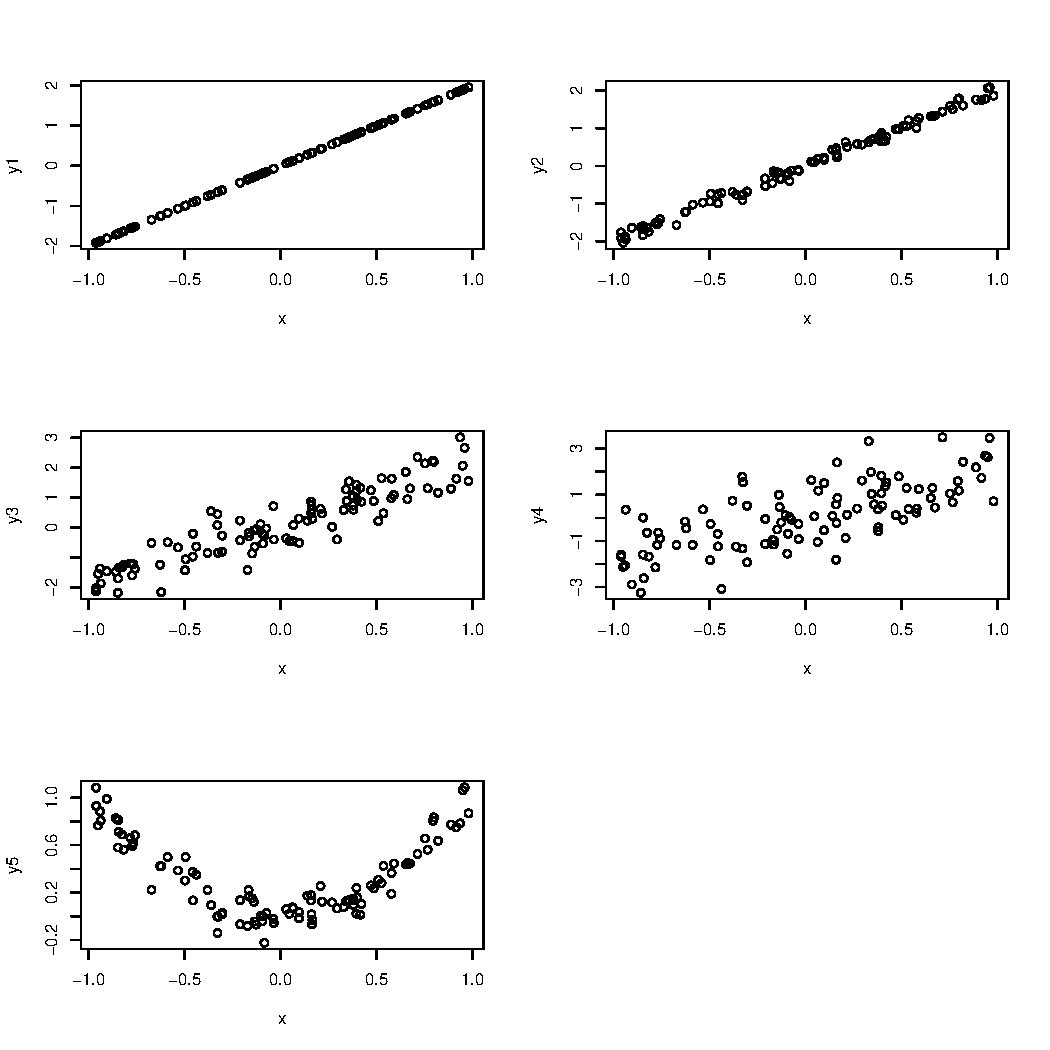
\includegraphics[page=1]{img/Lab3_1.pdf} 

\section*{Printout 2}
\addcontentsline{toc}{section}{Second Printout}

	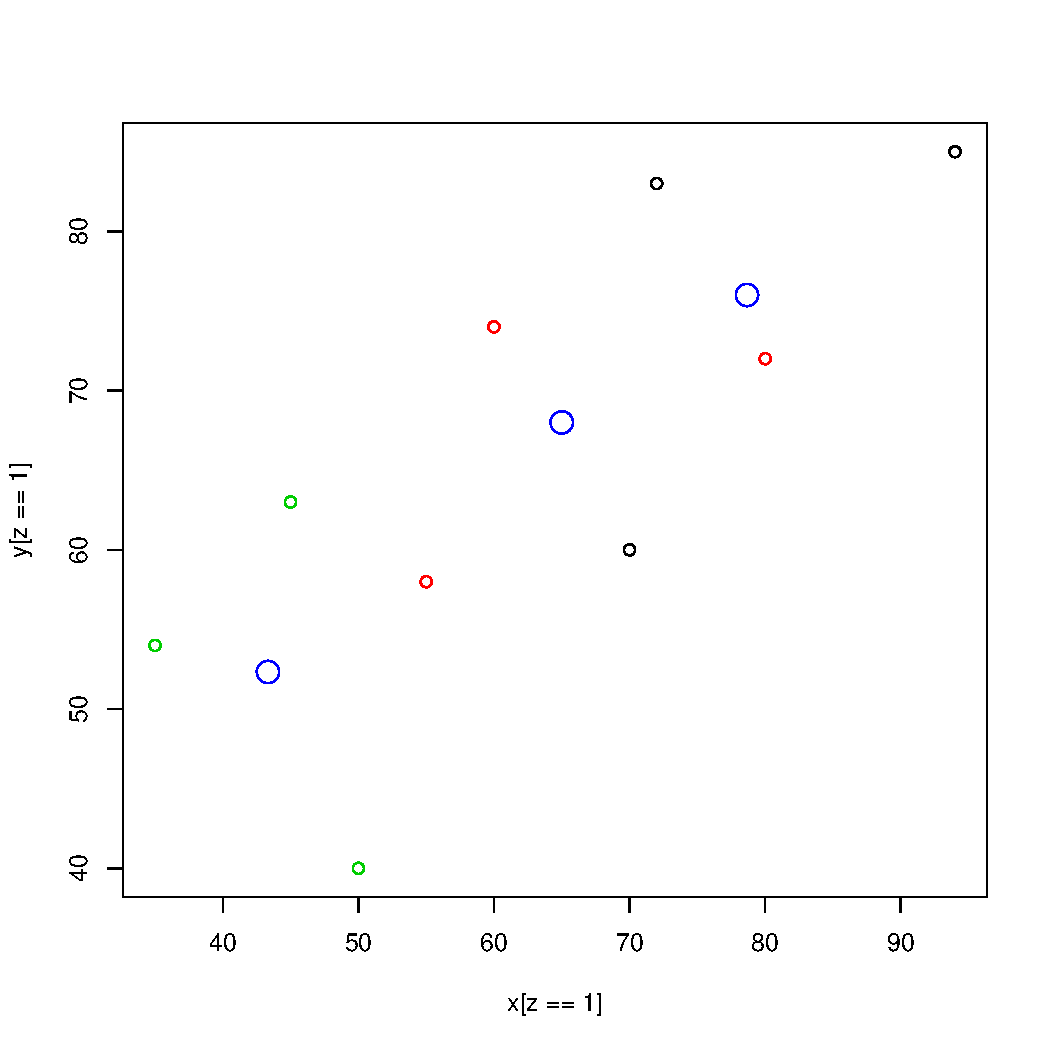
\includegraphics[page=1]{img/Lab3_2.pdf} 

\section*{Printout 3}
\addcontentsline{toc}{section}{Third Printout}

	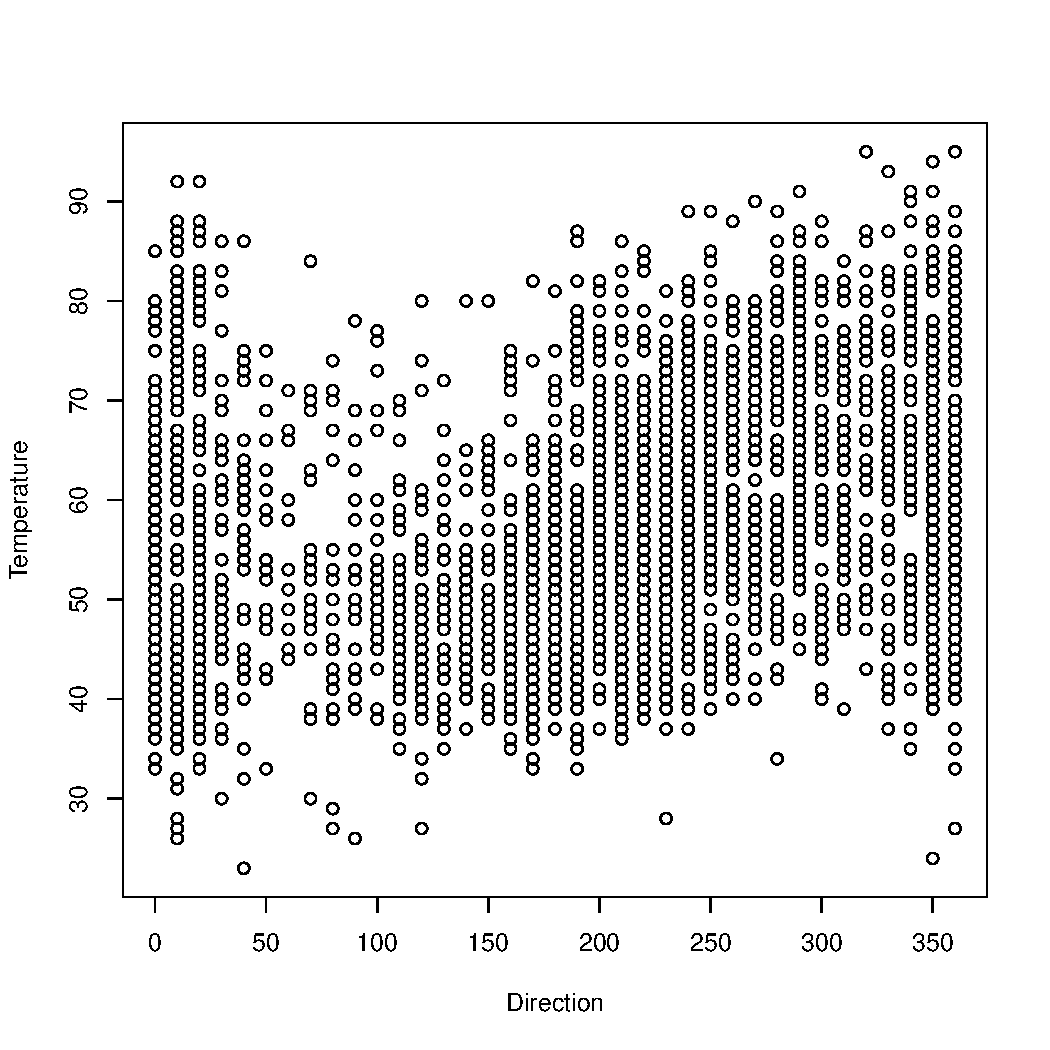
\includegraphics[page=1]{img/Lab3_3.pdf} 

	It appears that the relationship between temperature and wind direction is slightly positive 
	though, since there are so many data points that don't follow a certain pattern, there doesn't 
	really appear to be any correlation at all. It is also interesting to note that the values of wind 
	direction appear to be discrete because of how the data points are in columns rather than being 
	randomly scattered like the temperature.

\end{document}